\chapter{Recursive Methods}

\section{Tail Recursion}

Let's take another look at the \java{factorial} method from the book and its stack frames in Figure~\ref{fig.factorial_stack}.

\begin{code}
public static int factorial(int n) {
    if (n == 0) {
        return 1;
    }
    int recurse = factorial(n - 1);
    int result = n * recurse;
    return result;
}
\end{code}

\begin{figure}[!htb]
\begin{center}
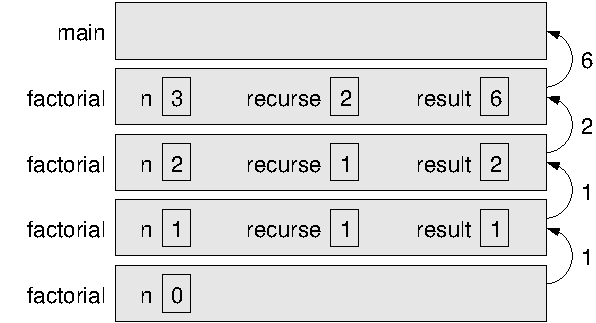
\includegraphics{figs/ch08/stack3.pdf}
\caption{Stack diagram for the \java{factorial} method.}
\label{fig.factorial_stack}
\end{center}
\end{figure}


The program can't calculate \java{factorial(3)} until it has figured out \java{factorial(2)}, which can't be calculated until \java{factorial(1)} is calculated, and so on.

This means that when the program gets to the base case, it has to return the result to the previous call, which has to return the result to {\em its} caller, passing results back up the call chain until the result is finally calculated. This process is indicated by the arrows in the diagram, and this is the process that tends to confuse people when they're learning about recursion.

On the other hand, look at \java{countdown} method and its stack frames in Figure~\ref{fig.countdown_stack}. 

\begin{code}
public static void countdown(int n) {
    if (n == 0) {
        System.out.println("Blastoff!");
    } else {
        System.out.println(n);
        countdown(n - 1);
    }
}
\end{code}

When the program hits the base case,  (\java{n == 0}) it's finished. There are no arrows in the diagram because there's no result to pass back to the previous caller; it's a \java{void} method.

\begin{figure}[!htb]
\begin{center}
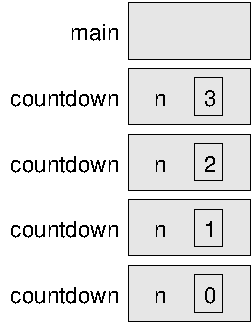
\includegraphics{figs/ch08/stack2.pdf}
\caption{Stack diagram for the \java{countdown} program.}
\label{fig.countdown_stack}
\end{center}
\end{figure}

This is why the book introduced recursion with the \java{countdown} method; it's conceptually simpler.

There is one other important difference between these two methods. In \java{countdown}, the recursive call is the very last thing that happens in the non-base case.  In \java{factorial}, the recursive call isn't the very last thing that happens. This is why the result has to be ``on hold'' until reaching the base case.

\index{tail recursion}
\index{recursion!tail}
When the recursive call is the very last thing that happens in the non-base case, the method is called a {\em tail recursive} method.

Even if you were to rewrite the \java{factorial} method in the following way, it would still {\em not} be tail recursive.

\begin{code}
public static int factorial(int n) {
    if (n == 0) {
        return 1;
    } else {
        return n * factorial(n - 1);
    }
}
\end{code}

In this version of the code, the recursive call to \java{factorial} still isn't the last thing that happens---the multiplication is the last operation.

Is it possible to write methods like \java{factorial} so that they use tail recursion? Yes, it is, by using something that I call the ``accumulator trick.'' We're going to write the method so that the accumulated result is one of the method parameters:

\begin{code}
public static int tailFactorial(int n, int result) {
    if (n == 0) {
        return result;
    } else {
        tailFactorial(n - 1, n * result);
    }
}
\end{code}

You call it like this:

\begin{code}
int fac3 = tailFactorial(3, 1); // initial value of result is 1
\end{code}

Let's see what happens when we call \java{tailFactorial(3, 1)}.

\vspace{-1ex}
\begin{quote}
\java{n} is 3 and \java{result} is 1. Since 3 is not 0, we call \java{tailFactorial(2, 3 * 1)}
\begin{quote}
\java{n} is 2 and \java{result} is 3. Since 2 is not 0, we call \java{tailFactorial(1, 2 * 3)}
\begin{quote}
\java{n} is 1 and \java{result} is 6. Since 1 is not 0, we call \java{tailFactorial(0, 6 * 1)}
\begin{quote}
\java{n} is 0 and \java{result} is 6. Since 0 {\em is} 0, we return the value of \java{result}, which is the correct answer: 6.
% without making any more recursive invocations.
\end{quote}
\end{quote}
\end{quote}
\end{quote}
\vspace{-1ex}

Once we hit the base case, we have the answer we want---it's passed all the way back up the chain.

Figure~\ref{fig.tail_recursive} shows the call stack for \java{tailFactorial}. You can think of the base case returning the accumulated result directly to the original caller.

\begin{figure}[!htb]
\begin{center}
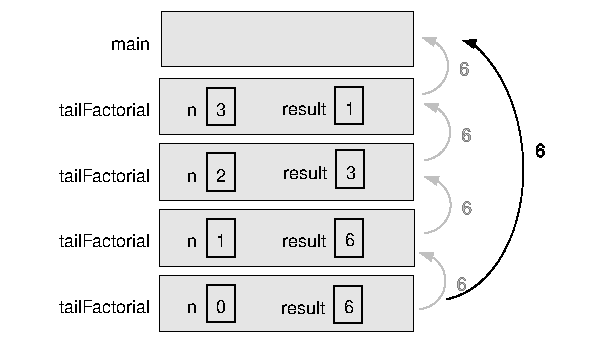
\includegraphics{figs/ch08/stack4.pdf}
\caption{Stack diagram for the \java{tailFactorial} program.}
\label{fig.tail_recursive}
\end{center}
\end{figure}

\index{tail call optimization}
\index{optimization!tail call} In fact, some languages, but {\em not} Java, do {\em tail call optimization}. Since all the necessary information is carried from stack frame to stack frame, these languages can optimize the code so that it re-uses the same stack frame over and over again. With this optimization, stack overflow cannot occur.

Even though Java doesn't do tail call optimization, you should still learn the ``accumulator trick.'' First, it's conceptually simpler: once you hit the base case, you've finished. Second, if you know how to write tail recursive methods in other languages that {\em do} optimize, you'll be in a position to take advantage of it.

\section{Overloaded Methods}
In the \java{tailFactorial} example, the user has to provide the number whose factorial they want as well as the starting value for the accumulator. We could make life easier for our users by providing a one-parameter \java{factorial} method for the convenience of our users:

\begin{code}
public int factorial(int n) {
    // Provide the result value
    // for the user's convenience
    return tailFactorial(n, 1); 
}
\end{code}

They would then be able to write code like this:

\begin{code}
int answer = factorial(7);
\end{code}

In this example, we have two different method names: \java{tailFactorial} and \java{factorial}. Many programming languages {\em require} you to have different names for all your methods. Java, however, is one of those languages which allow you to have multiple methods with the same name---as long as they have a different number and/or type of their parameters. This is called an {\em overloaded method}.

While overloading methods indiscriminately can lead to code that is difficult to read and maintain, overloading does have its place. For example, if you look at the documentation for the \java{Math} class at \url{https://docs.oracle.com/en/java/javase/16/docs/api/java.base/java/lang/Math.html}, you will see that the \java{Math.abs} method is overloaded to accept different data types.

We could write the preceding example to use overloading.

\begin{code}
 1 public static int factorial(int n, int result) {
 2     if (n == 0) {
 3         return result;
 4     } else {
 5         factorial(n - 1, n * result);
 6     }
 7 }
 8 
 9 public static int factorial(int n) {
10     factorial(n, 1);
11 }
12 
13 public static void main(String[] args) {
14     int answer = factorial(7);
15 }
\end{code}

When Java encounters the call on line 14, it sees there is only one parameter and calls the corresponding \java{factorial} method on line 9. When it gets to the call on line 10, it sees there are two parameters and calls the corresponding \java{factorial} method on line 1. The call on line 5 has two parameters, which means it is a recursive call to the method on line 1.

\section{Exercises}

\begin{exercise}
Find whether a \java{String} is a palindrome (the same forward and backwards, such as ``radar'' or ``racecar''). Write an \java{isPalindrome} method with this header:

\begin{code}
public static boolean isPalindrome(String s, int start, int end) 
\end{code}

where \java{s} is the string you are testing, \java{start} is the starting index in the string, and \java{end} is the ending string.

If the characters at the \java{start} and \java{end} position are not identical, return \java{false}; it's not a palindrome. Otherwise, \java{return} the result of a recursive call to \java{isPalindrome}, adding one to the \java{start} position and subtracting one from the \java{end} position.

The base case occurs when the \java{start} and \java{end} position are the same, which happens for words like ``radar``, or when \java{start} becomes greater than \java{end}, which happens for words like ``anna''. If you reach the base case, return \java{true}.

As described here, this is a naturally tail recursive process. Either it fails on a mismatch, or you hit the base case and you've finished.

\end{exercise}


\begin{exercise}
Write a tail recursive method to find the sum of an array of integers. To use the accumulator trick in this method, you'll need to keep track of {\em two} things: one for the current index into the array and another for the accumulated sum, which starts at 0. The base case occurs when the index equals the array length; at that point you have the result in the accumulated sum. The method header might look like this:

\begin{code}
public static int sum(int[] arr, int index, int sum)
\end{code}

You would call it like this:

\begin{code}
int[] data = {10, 47, 66, 11};
int total = sum(data, 0, 0);
\end{code}

\end{exercise}

\begin{exercise}
Write a tail recursive method to find the {\em n}th Fibonacci number. To use the accumulator trick in this method, you'll need to keep track of which Fibonacci number you're working on ({\em hint}: it counts down), the current result, and the previous result. The method header might look like this:

\begin{code}
public static int fibonacci(int n, int result, int previous)
\end{code}

The base case occurs when \java{n} is 1 or 2, in which case you return 1.

You would call it like this:

\begin{code}
// Find the twelfth Fibonacci number
int answer = fibonacci(10, 1, 1); // should be 55
\end{code}

\end{exercise}

\begin{exercise}
In order to make your methods more friendly to users, use method overloading to implement these methods for the preceding exercises:

\begin{itemize}
\item \java{public static boolean isPalindrome(String s)}
\item \java{public static int sum(int[] arr)}
\item \java{public static int fibonacci(int n)}
\end{itemize}
\end{exercise}
